\documentclass[10pt]{article}
\usepackage[utf8]{inputenc}
\usepackage{pgfplots}
\pgfplotsset{compat=1.15}
\usepackage{mathrsfs}
\usetikzlibrary{arrows}
\pagestyle{empty}
\begin{document}
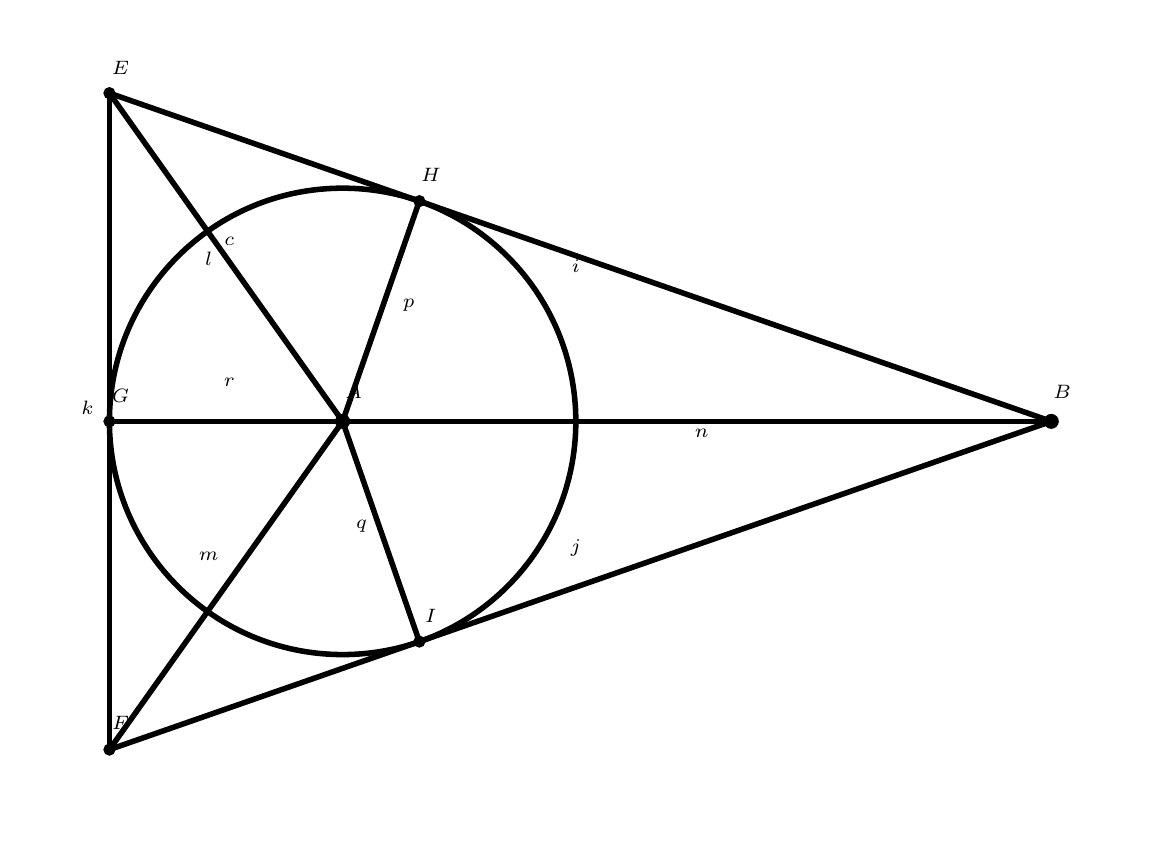
\begin{tikzpicture}[line cap=round,line join=round,>=triangle 45,x=1.0cm,y=1.0cm]
\clip(-4.,-5.) rectangle (10.,5.);
\draw [line width=2.pt] (0.,0.) circle (2.961688707477543cm);
\draw [line width=2.pt] (-2.961688707477543,4.168481786721364)-- (9.,0.);
\draw [line width=2.pt] (9.,0.)-- (-2.961688707477543,-4.168481786721364);
\draw [line width=2.pt] (-2.961688707477543,4.168481786721364)-- (-2.961688707477543,-4.168481786721364);
\draw [line width=2.pt] (-2.961688707477543,4.168481786721364)-- (0.,0.);
\draw [line width=2.pt] (0.,0.)-- (-2.961688707477543,-4.168481786721364);
\draw [line width=2.pt] (0.,0.)-- (9.,0.);
\draw [line width=2.pt] (0.,0.)-- (0.9746222222222218,2.7967322939370898);
\draw [line width=2.pt] (0.,0.)-- (0.9746222222222218,-2.7967322939370898);
\draw [line width=2.pt] (0.,0.)-- (-2.961688707477543,0.);
\begin{scriptsize}
\draw [fill=black] (0.,0.) circle (2.5pt);
\draw[color=black] (0.14,0.37) node {$A$};
\draw[color=black] (-1.44,2.29) node {$c$};
\draw [fill=black] (9.,0.) circle (2.5pt);
\draw[color=black] (9.14,0.37) node {$B$};
\draw [fill=black] (-2.961688707477543,4.168481786721364) circle (2.0pt);
\draw[color=black] (-2.82,4.49) node {$E$};
\draw [fill=black] (-2.961688707477543,-4.168481786721364) circle (2.0pt);
\draw[color=black] (-2.82,-3.83) node {$F$};
\draw[color=black] (2.96,1.97) node {$i$};
\draw[color=black] (2.96,-1.61) node {$j$};
\draw[color=black] (-3.24,0.17) node {$k$};
\draw [fill=black] (-2.961688707477543,0.) circle (2.0pt);
\draw[color=black] (-2.82,0.33) node {$G$};
\draw [fill=black] (0.9746222222222218,2.7967322939370898) circle (2.0pt);
\draw[color=black] (1.12,3.13) node {$H$};
\draw [fill=black] (0.9746222222222218,-2.7967322939370898) circle (2.0pt);
\draw[color=black] (1.12,-2.47) node {$I$};
\draw[color=black] (-1.7,2.07) node {$l$};
\draw[color=black] (-1.7,-1.71) node {$m$};
\draw[color=black] (4.56,-0.15) node {$n$};
\draw[color=black] (0.84,1.47) node {$p$};
\draw[color=black] (0.24,-1.33) node {$q$};
\draw[color=black] (-1.44,0.49) node {$r$};
\end{scriptsize}
\end{tikzpicture}
\end{document}